
\noindent\chenkai{colored sentences were added/modified/highlighted according to comments}


% \begin{figure*}
% 	\begin{center}
% 		\centerline{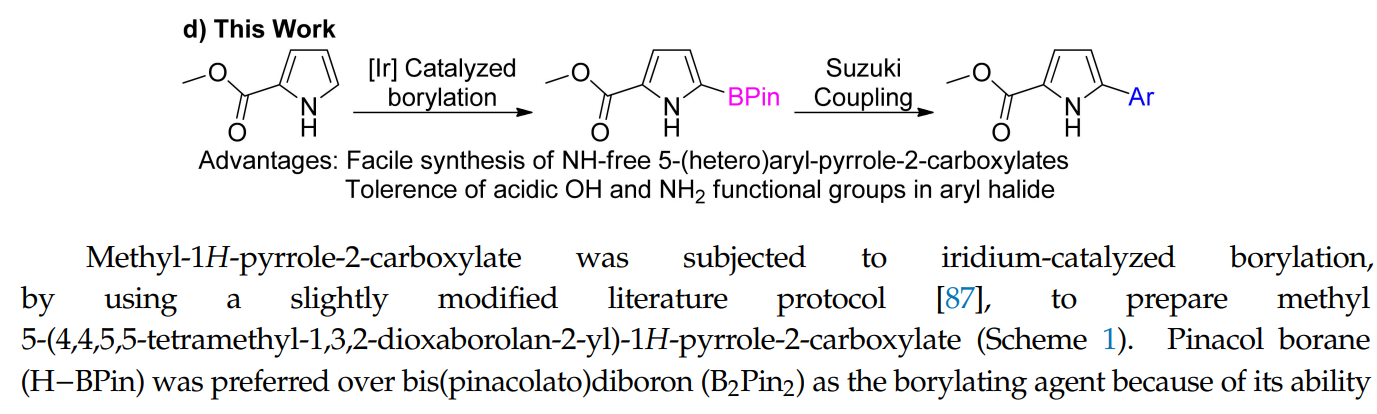
\includegraphics[width=2
% 			\columnwidth]{screenshot.png}}
% 		\caption{An screenshot of a portion of chemistry article~\cite{chem_article}. The text involves chemical formula, reaction, and complex chemical names.}
% 		\label{fig:screenshot}
% 	\end{center}
%  	\vskip -0.2in
% \end{figure*}

\section{Introduction}
\label{intro}
%\cite{abdalla-teufel-2006-bootstrapping}

% \heng{1.emphasize there is little NLP work for Chemistry domain; you propose a novel problem formulation and a potential solution; 2. walk through some examples when explaining the characteristics; 3. explain the main challenges to discuss the difference between Biomedical and chemistry domains; 4. distant supervision for training data acquisition; 5. for the walk-through example try to }

% \heng{only use 'work' instead of 'works', and use present tense instead of past tense}
% \heng{Explain why fine-grained entity typing is important for this domain, and what it is by giving a challenging example at teh beginning. } \cheng{I agree that a specific example at the very beginning would be very useful. We can use the example to make all the major (general) points we want to make. Perhaps a sample text, chemical structure and a target concept in an ontology?}
%Information extraction refers to the task of transforming text into structured knowledge elements, which is a crucial step for many downstream tasks, such as %knowledge graph construction and 
%question answering. 
As the amount of research literature is growing exponentially, accurate and efficient information extraction (IE) methods are crucial for many downstream applications including question answering and knowledge reasoning. One  domain largely overlooked by previous IE research is Chemistry (an example sentence is shown in Figure~\ref{fig:framework}), which consists of discussion on chemicals and reactions they are involved. What benefit can it bring if we develop well-performing IE methods for chemistry domain? If a comprehensive chemistry knowledge base can be efficiently constructed, chemicals can be discovered at a faster pace since models can learn from existing reactions to infer never-imagined ones, thus benefiting downstream applications such as those in biomedical research and chemical industry.  
% (a screenshot of a chemistry paper is shown in Figure~\ref{fig:screenshot})
%indispensable for structurizing text automatically in order to enrich knowledge base, which many inference tasks that require reasoning depend on. 
% COMMENTS
% \heng{simply say domain knowledge is too vague, need to elaborate it clearly: multi-modal representation, external knowledge via entity linking}

One fundamental building-block of information extraction is fine-grained entity typing (FET), which is the task of classifying entity mentions into subset of pre-defined hierarchical classes (e.g., Person/Artist, Location/City in news domain), and doing well in such task typically requires the system to understand the mention and its context well.
The task is particularly challenging for scientific articles, where domain-specific knowledge is heavily required to understand the text; for instance, in chemistry, one needs to understand the reaction mechanism in the literature described by both equation image and text (about experiment conditions), and since a reaction is based upon chemical compounds, it additionally assumes one to have knowledge about the chemical as well. Intuitively, to understand scientific articles, linking entities appearing in the text to retrieve and comprehend external information in different modalities would be very helpful. Analogically, when a person learns a cooking recipe, he or she would look up cooking instruction video (consisting of image, text, and audio) to help understanding the procedure In scientific domains, information extraction models have been widely developed for biomedical context~\cite{biomedie, biomedpp1, biomedpp2, biomedpp3, biomedpp4, scibert,biobert, biomedpp5,biomedpp6}  However, while chemistry research shapes the foundation of many biomedical studies, there has been little work done in extracting knowledge from core chemistry research literature; previous work in Chemistry IE mainly focuses on Named Entity Recognition (NER) (e.g., recognizing chemical name spans), and there is only one work we were able to find~\cite{chemu} on task other than NER (e.g., reaction event extraction). One major difference between chemistry and biomedical literature text lies in different chemical entity expressions, where chemical compounds in biomedical text are often expressed in natural language (e.g., water, aspirin), while in chemistry it's often complex formula-like names (e.g., 5,6-dihydroxycyclohexa-1,3-diene-1-carboxylic acid, H2O), which is hard to be understood by existing language models as such complex names do not follow morphological structure like other commonly used words like ``basketball''. To make the situation worse, many chemicals simply have never been coined with any nomenclature in natural language. The chemical mentions are essentially rare terms that is not best to be  and thus would be not learned well by language model  

%COMMENT
%  \heng{add more recent citations}

% Even if we pre-trained on these complex synonyms, most chemical entities would still be 

% COMMENTS
% \cheng{this point could be moved earlier to stress the importance of IE for chemistry domain. Perhaps we can first motivate IE in the literature in general and then say IE for Chemistry is especially important for reasons of xx, yy? Logically, it seems natural to first motivate the general problem of IE, then motivate the entity typing in general, and finally fine-grained typing. We can then discuss the unique challenges of fine-grained typing that make existing approaches to typing inadequate. We propose to use multimodal knowledge representation to address the (unique) challenges. In the experiment part, we can then show the proposed approach is indeed effective for addressing the new challenges (e.g., by showing cases where SOTA methods failed, but the proposed approach succeeded.}
%, thus benefiting different parties, including biomedical studies and chemical industries.
% In this work, we explore fine-grained chemical typing, which is the task of classifying chemical mentions into fined-grained types. 
% COMMENTS
% \cheng{Need to briefly mention existing methods to entity-typing here and why they may be inadequate for the chemical fine-grained typing. Is it because of the challenge associated with Chemistry or the ``fine-grained" typing. In general, it might be good to say something like "Our (new) task poses several (unique/new?) challenges: (a) Chemsitry domain... (b) fine-grained (vs. coarse grained)..... It would be great to clarify which is the major challenge that we focus on tackling. } 


% COMMENTS
% \cheng{Is it possible to coin a new name for ``this promising field"? Or otherwise be specific, e.g.,  ``Chemical Information Extraction"? Is this term already standard? Or perhaps "Chemical Knowledge Base Population"? }
Although there has been a line of method in FET applied to news domain~\cite{ultrafet, label_bias, fet_el, lin2019attentive,hierarchical_gcn, hyperbolic}, none have been developed for core chemistry literature and they do not consider any types of domain-specific knowledge. While language model may have a hard time understand the chemical mention purely based on its surface form and contextual representation, we can understand the identity through it's external information (in different modalities) such as natural language description about its properties and it's structure (or graph). In the chemical typing task particularly, compound types can be well correlated with properties and physical structure 
% COMMENTS

% \heng{use this to motivate why text-only representation is not enough}  
%in chemical literature, which potentially improves the understanding of chemical mention and learn correlation between different entities.
% , we see the urgent need of a line of benchmark datasets and methods to encourage people to drive this promising field, \bluetext{Chemistry Information Extraction (ChemIE)}.
% While general domain language model can be massively pre-trained upon external text to achieve a good performance in chemical entity classification, they miss incorporate different modalities of information, such as chemical structures. 

% COMMENTS

% \heng{need to emphasize the novelty of the work: multimodal information, incorporating external knowledge}
% \cheng{it would also be good to discuss the generality of the novelty. Is the novelty specific to the particular problem/task or Chemical domain? Or perhaps it's novel in the context of typing? Clarifying the scope of novelty would be helpful. It can either help ``defend" the novelty if it's only specific to Chem IE, or help ``amplify" the novelty/impact if it's not just restricted to Chem IE.} 
% \heng{for paper writing, use present tense instead of past tense for both of your work and related work}
Our work is novel in that we are the very pioneers to explore FET strategies in chemistry. Utilizing external database for multimodal information retrieval, we introduce a deep learning based method that use cross-modal attention to align and embed the structure and description text of chemicals into a common space as core features for classification. %, which under the shell aims to align properties phrase and molecule substructure.
As illustrated in Figure~\ref{fig:intuition}, %intuitively,
some patterns of molecular substructures well align with the phrases in description text. For example the circled sub-structure in the is commonly appeared together with  "polar aprotic".

% comment
% \heng{I commented out the following sentence because it's very confusing, need to re-write:}

%The addition of multiple modalities targets achieving the same goal as image-text co-embedding, that is, to build a unified representation that allows reasoning over different perceptions; such representation can result in more discriminative predictions, which is shown in our experiments.


% comment

% \cheng{"limited dataset" is a bit vague. I think we can say more definitely that there doesn't already exist such a data set, right? I'm thinking of something like ``Since the proposed task has not been studied in the previous work, there is no dataset available for evaluating the task. To facilitate the study of this new task, we construct the first data set for fine-grained typing in the chemistry literature domain..... .}
Since the proposed task has not been studied in the previous work, there is no dataset available for evaluating the task. To facilitate the study of this new task, we construct CHEMET\footnote{Both the dataset and the code will be released to public}, the first dataset for fine-grained typing in the chemistry literature domain, for which we referred to wikipedia category for ontology construction, and used distant supervision to generate training data and facilitate annotation procedure. The dataset was based upon a corpus of 50 open access papers from a database on a specific theme. We will discuss the data construction details in Section \ref{datacollection}. Experimental results on the the dataset show that our method outperforms the state-of-the-art methods in entity typing. To the best of our knowledge, our method is the first to take step toward tackling fine-grained chemical entity typing.

% Since there is no dataset available for chemical FET, we have collected and annotated a new dataset, 

%  We will release the dataset in our code repository. 

Overall, our contributions can be summarized as the following:
% comment

% \heng{convert these into bullets} 
% \heng{the following bullets need to be re-written in a more concise and formal way}


\begin{itemize}
    \item We study the task of fine-grained chemical entity typing in chemistry literature, a largely under-explored yet promising field for NLP that has a great need for information extraction methods
    \item We construct the first human-annotated dataset in  fine-grained chemical entity typing and will release to the public.
    \item We introduce an novel method that utilizing multimodal knowledge representation to enrich entity mention representation
    \item The multimodal component of the model is based on structure and text alignment, which has never been explored before and can be applied to variety of ChemIE tasks such as relation extraction and event extraction.
    \item Experiments on the dataset show that our model outperforms the state-of-the-arts entity typing models. 
\end{itemize}




% that has a great needs information extraction methods in order to conduct experiments more efficiently

% \st{In this work, we explored relation extraction, the task of classifying 
%relationship between named entities (given by the task) into a subset of 
%predefined classes. Since there is no existing chemical benchmark on 
%information extraction, we also release a  dataset on named entity 
%recognition, 
%relation extraction, and event extraction, based on chemistry research 
%articles 
%on diverse topics. The ontology was carefully crafted in collaboration with 
%chemistry authorities, and data samples are annotated by chemistry students. 
%The dataset was designed in hope of encouraging further development of 
%information extraction methods on chemistry literature. In short, we made the 
%following contributions:...}





\begin{figure}
 	\vskip 0.2in
	\begin{center}
		\centerline{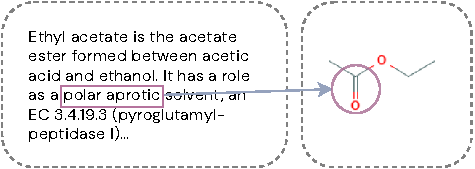
\includegraphics[width=0.9 
			\columnwidth]{intuition.pdf}}
		\caption{An example of chemical entity structure aligning with textual concepts. The circled sub-structure is
		often induce the "polar aprotic" property
% 		commonly described by polar aprotic"
		infer that ethyl acetate is polar aprotic}
		\label{fig:intuition}
	\end{center}
 	\vskip -0.2in
\end{figure}